% Process (how the work will be performed)
\chapter{Processo (como o trabalho ser� realizado)}

% Maintainer?s process (give an overview of the process, do not spell out the entire process in the maintenance plan)
\section{Processo de manuten��o (d� uma vis�o geral do processo, n�o especifique a totalidade processo no plano de manuten��o)}
\begin{figure}[h!]
	\caption{Framework Scrum}
	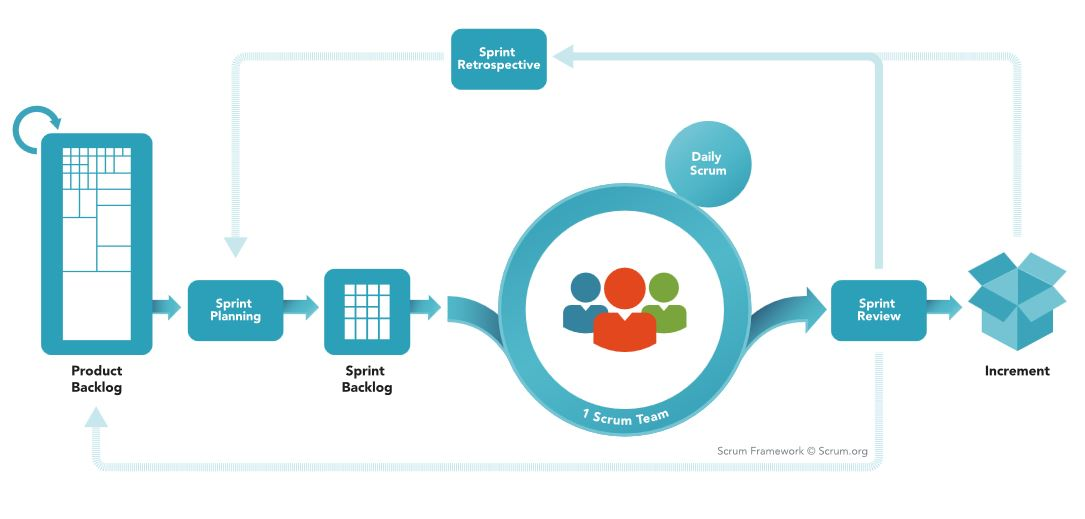
\includegraphics[width=\textwidth]{./h/scrum.jpg}
	\fonte{https://www.scrum.org/resources/what-is-scrum}
\end{figure}

% Defined process (identify actions to be performed for each activity in the process)
\section{Processo definido (identificar a��es a serem realizadas para cada atividade no processo)}
\begin{itemize}
	\item Backlog da manuten��o: Reuni�o para definir as modifica��es necess�rias.
	\item Sprint Backlog: Reuni�o de planejamento do Sprint.
	\item Implementa��o.
	\item Reuni�es apenas semanais do Scrum, para an�lise do que j� foi feito e do que ainda falta.
	\item Reuni�o de Review do Sprint para definir se a implementa��o ser� aceita.
	\item Reuni�o de Retrospectiva do Sprint para definir o que pode ser melhorado no processo.
\end{itemize}